\subsubsection{LiteDB Pipeline} \label{sec:ExperimentePIPE}
    Um die Suche von mehreren Paketen in der Datenbasis zu beschleunigen wurde sich das Prinzip der Parallelisierung zu Nutzen gemacht.
    Hierzu wurde die zu untersuchende Liste von Paketen auf verschiedene Tasks aufgeteilt.
    So ist nach dem vollständigen Befüllen der Pipeline eine theoretischen Laufzeitverkürzung um der Faktor der maximal abarbeitbaren Tasks erreicht.  
    
    Dabei sind zwei Fälle zu unterscheiden:
    \begin{description}
        \item[\textit{Weniger} Pakete als Datenbank-Dateien]\hfill \\
            In diesem Falle einer geringeren Anzahl an Pakete wird die Pipe nie vollständig gefüllt.
        \item[\textit{Mehr} Pakete als Datenbank-Dateien]\hfill \\
            In jenem Falle muss die Paketliste Stück für Stück in die Pipe eingefügt werden und beim Erreichen der Kapazität -- entsprechend der Anzahl der Datenbanken -- das früheste Paket entfernt und ein neues Paket am Anfang eingefügt werden.
    \end{description}
    
    Die Verwaltung der 3 verschiedenen Staaten der Pipe ist in folgender Abbildung mit \ac{PAP} nachvollziehbar.
    Anschließend sind die 3 Fälle näher ausgeführt.
    \begin{figure}[H]
        \centering
        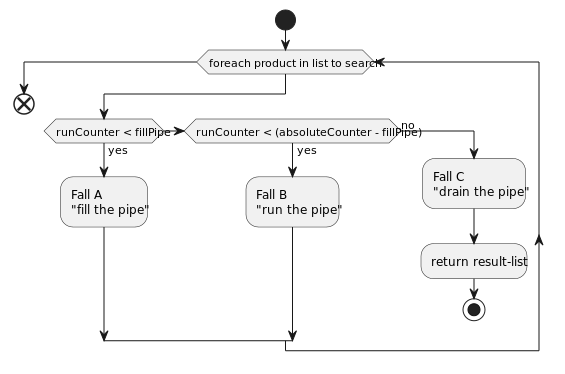
\includegraphics[width=\textwidth]{../pap/Simultanius search on LiteDb-Files.png}
        \caption{Übersicht der Pipeline-Staaten}
        \label{png:OverviewPipelineStatus}
    \end{figure}

    Das Befüllen der Pipeline geschieht nach folgendem Muster:
    \begin{figure}[H]
        \centering
        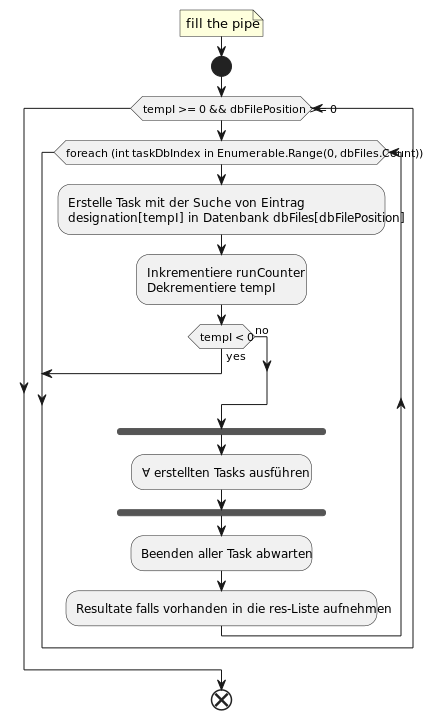
\includegraphics[width=\textwidth]{../pap/Case_A.png}
        \caption{\ac{PAP} Befüllen der Pipeline}
        \label{png:case_a}
    \end{figure}

    Nach vollständiger Befüllung die Erhaltung der Pipeline:
    \begin{figure}[H]
        \centering
        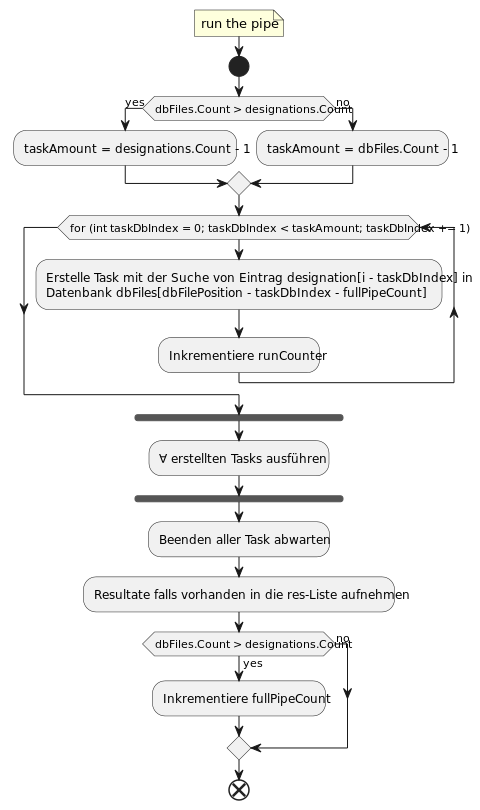
\includegraphics[width=\textwidth]{../pap/Case_B.png}
        \caption{\ac{PAP} Aufrechterhalten der Pipeline}
        \label{png:case_b}
    \end{figure}

    Beim Leeren der Pipeline:
    \begin{figure}[H]
        \centering
        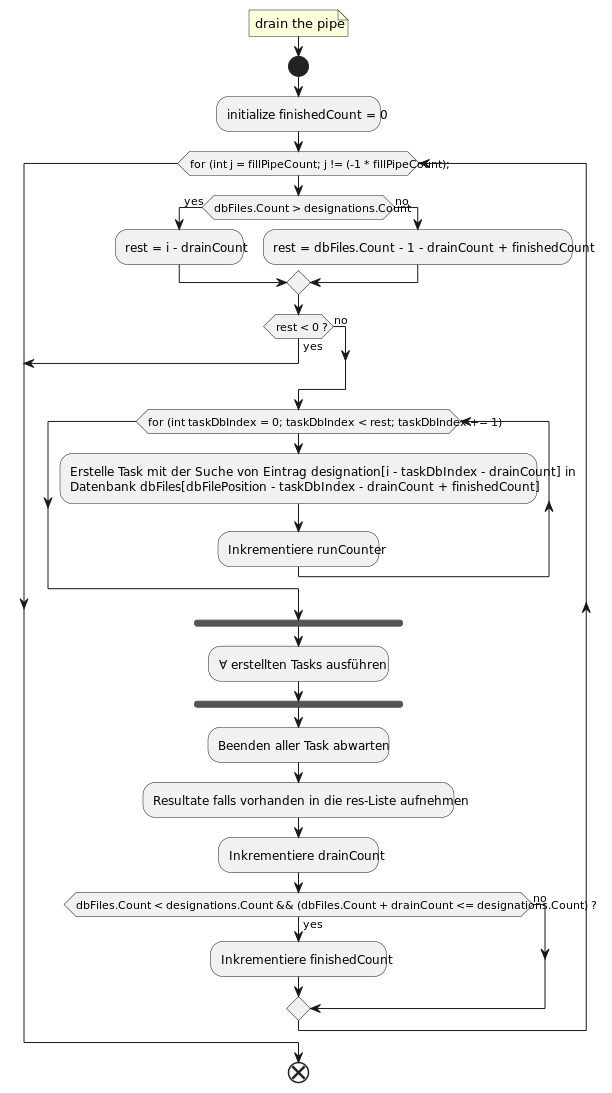
\includegraphics[width=\textwidth]{../pap/Case_C.png}
        \caption{\ac{PAP} Leeren der Pipeline}
        \label{png:case_c}
    \end{figure}

    Aus der Implementation der Pipeline ergeben sich folgende Laufzeiten bei weniger Paketen als Datenbankdateien:
    \begin{tabular}{|c|c|c|}
        \hline
            Such-Typ & Zeit & Faktor \\
            Mono-Suche & 262676.7ms & 1 \\
            Pipeline & 96868.4ms & 2.7213448 \\
        \hline
    \end{tabular}

    Aus der Implementation der Pipeline ergeben sich folgende Laufzeiten bei weniger Paketen als Datenbankdateien:
    \begin{tabular}{|c|c|c|}
        \hline
            Such-Typ & Zeit & Faktor \\
            Mono-Suche & 95011.24ms & 1 \\
            Pipeline & 22111.5ms & 4.296846569 \\
        \hline
    \end{tabular}
